\documentclass[12pt]{article}
\usepackage[paper=letterpaper,margin=2cm]{geometry}
\usepackage{amsmath}
\usepackage{amssymb}
\usepackage{amsfonts}
\usepackage{newtxtext, newtxmath}
\usepackage{enumitem}
\usepackage{titling}
\usepackage{svg}
\usepackage{xcolor}
\usepackage{listings}
\usepackage{float}
\usepackage{paracol}
\usepackage{nicefrac}
\usepackage{ragged2e}
\usepackage[autostyle]{csquotes}
\usepackage[colorlinks=true]{hyperref}

\MakeOuterQuote{"}
\setlength{\droptitle}{-6em}

\definecolor{codegreen}{rgb}{0,0.6,0}
\definecolor{codegray}{rgb}{0.5,0.5,0.5}
\definecolor{codepurple}{rgb}{0.58,0,0.82}
\definecolor{backcolour}{rgb}{0.95,0.95,0.92}

\lstdefinestyle{mystyle}{
    commentstyle=\color{codegreen},
    keywordstyle=\color{magenta},
    numberstyle=\tiny\color{codegray},
    stringstyle=\color{codepurple},
    basicstyle=\ttfamily\footnotesize,
    breakatwhitespace=false,
    breaklines=true,
    captionpos=b,
    keepspaces=true,
    numbers=left,
    numbersep=5pt,
    showspaces=false,
    showstringspaces=false,
    showtabs=false,
    tabsize=2
}

\lstset{
        style=mystyle,
        inputencoding=utf8,
        extendedchars=true,
}


\newcommand{\me}{\mathrm{e}}

\title{\large{Aprendizagem 2022}\vskip 0.2cm Homework IV -- Group 019\vskip 0.2cm Diogo Gaspar 99207, Rafael Oliveira 99311}
\date{}
\begin{document}
\maketitle
\center\large{\vskip -2.5cm\textbf{Part I}: Pen and paper}
\begin{enumerate}[leftmargin=\labelsep]

  \item \textbf{Perform one epoch of the EM clustering algorithm and determine the new parameters.}

        As a side note, we'll be using the $k_1$ and $k_2$ notation to represent
        clusters $1$ and $2$ - with that, we'll say that $\pi_1 = P(C = k_1)$,
        with analogous notation for $\pi_2$.

        EM-Clustering, being an unsupervised learning algorithm intending to calculate
        the probability of a sample belonging to a certain cluster, is a method that
        iteratively updates the parameters of the model until convergence is reached
        (for a given definition of convergence). Here, we'll perform exactly one
        epoch of the algorithm, which means we'll be going through two steps:

        \begin{itemize}[leftmargin=\labelsep]
          \item \textbf{E-step:} In this step, our goal is to calculate the \textbf{posterior
                  probability} of each sample belonging to each cluster.
                In order to perform this calculation, we'll be using \textbf{Bayes' rule},
                of course, to decompose the posterior probability into the product of
                the \textbf{likelihood} and the \textbf{prior probability} of the sample
                belonging to the cluster. Let's try, then, to assign each sample to
                the cluster that maximizes the posterior probability.

                For starters, we must first note that the likelihood of a sample
                belonging to a cluster is given by the \textbf{multivariate Gaussian
                  distribution}, which can be written as (considering $d = 2$, as we
                are working with two dimensions here):

                \begin{equation*}
                  P(x_i \mid C = k_n) \sim \mathcal{N}(x_i; \mu_n, \Sigma_n) = \frac{1}{\sqrt{(2\pi)^d \det \Sigma_n}}
                  \exp \left( -\frac{1}{2} (x_i - \mu_n)^T \Sigma_n^{-1} (x_i - \mu_n) \right)
                \end{equation*}

                We'll also use the $\gamma_{i, j}$ notation to represent the normalized
                posteriors, where $i$ matches the $i$-th sample and $j$ the $j$-th cluster
                (considering $N = 2$, as we have two clusters $k_\alpha, \forall_{1 \leq \alpha \leq N}$):

                \begin{equation*}
                  \gamma_{i, j} = P(C = k_j | x_i) = \frac{\pi_j P(x_i \mid C = k_j)}{\sum_{\alpha=1}^N \pi_\alpha P(x_i \mid C = k_\alpha)}
                  = \frac{\pi_j \mathcal{N}(x_i; \mu_j, \Sigma_j)}{\sum_{\alpha=1}^N \pi_\alpha \mathcal{N}(x_i; \mu_\alpha, \Sigma_\alpha)}
                \end{equation*}

                Moreover, in this step we'll use \textcolor{teal}{teal} to denote the priors and
                \textcolor{purple}{purple} to denote the likelihoods.

                \pagebreak

                As a given, we have that the priors are (for every sample, of course):

                \begin{equation*}
                  \textcolor{teal}{P(C = k_1)} = \textcolor{teal}{P(C = k_2)} = \pi_1 = \pi_2 = 0.5
                \end{equation*}

                Regarding $x_1$, we have:

                \begin{equation*}
                  \begin{aligned}
                    \textcolor{purple}{P(x_1 \mid C = k_1)}
                     & = \frac{1}{\sqrt{(2\pi)^d \det \Sigma_1}} \exp \left( -\frac{1}{2} (x_1 - \mu_1)^T \Sigma_1^{-1} (x_1 - \mu_1) \right)                                                                                \\
                     & = \frac{1}{\sqrt{(2\pi)^2 \det \begin{bmatrix}
  2 & 1\\
  1 & 2\\
\end{bmatrix}}}
                    \exp \left( -\frac{1}{2} \left(\begin{bmatrix}
  1.19722 & 1.2214 & 1.24608\\
  1.19722 & 1.2214 & 1.24608\\
\end{bmatrix} - \begin{bmatrix}
  2\\
  2\\
\end{bmatrix}\right)^T \begin{bmatrix}
  2 & 1\\
  1 & 2\\
\end{bmatrix}^{-1} \left(\begin{bmatrix}
  1.19722 & 1.2214 & 1.24608\\
  1.19722 & 1.2214 & 1.24608\\
\end{bmatrix} - \begin{bmatrix}
  2\\
  2\\
\end{bmatrix}\right) \right) \\
                     & \approx 0.0658407
                  \end{aligned}
                \end{equation*}

                \begin{equation*}
                  \begin{aligned}
                    \textcolor{purple}{P(x_1 \mid C = k_2)}
                     & = \frac{1}{\sqrt{(2\pi)^d \det \Sigma_2}} \exp \left( -\frac{1}{2} (x_1 - \mu_2)^T \Sigma_2^{-1} (x_1 - \mu_2) \right)                                                                                \\
                     & = \frac{1}{\sqrt{(2\pi)^2 \det \begin{bmatrix}
  2 & 0\\
  0 & 2\\
\end{bmatrix}}}
                    \exp \left( -\frac{1}{2} \left(\begin{bmatrix}
  1.19722 & 1.2214 & 1.24608\\
  1.19722 & 1.2214 & 1.24608\\
\end{bmatrix} - \begin{bmatrix}
  0\\
  0\\
\end{bmatrix}\right)^T \begin{bmatrix}
  2 & 0\\
  0 & 2\\
\end{bmatrix}^{-1} \left(\begin{bmatrix}
  1.19722 & 1.2214 & 1.24608\\
  1.19722 & 1.2214 & 1.24608\\
\end{bmatrix} - \begin{bmatrix}
  0\\
  0\\
\end{bmatrix}\right) \right) \\
                     & \approx 0.0227993
                  \end{aligned}
                \end{equation*}


                The (normalized) posteriors can be computed as follows:

                \begin{equation*}
                  \begin{aligned}
                    \gamma_{1, 1} & = \frac{\textcolor{teal}{P(C = k_1)} \textcolor{purple}{P(x_1 \mid C = k_1)}}{\textcolor{teal}{P(C = k_1)} \textcolor{purple}{P(x_1 \mid C = k_1)} + \textcolor{teal}{P(C = k_2)} \textcolor{purple}{P(x_1 \mid C = k_2)}} \\
                                  & = \frac{0.5 \cdot 0.0658407}{0.5 \cdot 0.0658407 + 0.5 \cdot 0.0227993}                                                                                                                                                    \\
                                  & = 0.742788
                  \end{aligned}
                \end{equation*}

                \begin{equation*}
                  \begin{aligned}
                    \gamma_{1, 2} & = \frac{\textcolor{teal}{P(C = k_2)} \textcolor{purple}{P(x_1 \mid C = k_2)}}{\textcolor{teal}{P(C = k_1)} \textcolor{purple}{P(x_1 \mid C = k_1)} + \textcolor{teal}{P(C = k_2)} \textcolor{purple}{P(x_1 \mid C = k_2)}} \\
                                  & = \frac{0.5 \cdot 0.0227993}{0.5 \cdot 0.0658407 + 0.5 \cdot 0.0227993}                                                                                                                                                    \\
                                  & = 0.257212
                  \end{aligned}
                \end{equation*}

                \pagebreak

                As to avoid presenting here the repetitive calculations for the remaining samples,
                for which the results in question are calculated in the same manner, we include here
                only the intermediate values of such calculations, as discussed with Prof. Rui
                Henriques. The respective Python code is available in this report's appendix.

                \begin{paracol}{2}
                  \setlength{\columnseprule}{1pt}
                  \def\columnseprulecolor{\color{black}}
                  \centering

                  $x_2$:

                  \begin{equation*}
                    \begin{aligned}
                      \textcolor{purple}{P(x_2 | C = k_1)} & = 0.00891057 \\
                      \textcolor{purple}{P(x_2 | C = k_2)} & = 0.0482662
                    \end{aligned}
                  \end{equation*}

                  \begin{equation*}
                    \begin{aligned}
                      \gamma_{2, 1} & = 0.155843 \\
                      \gamma_{2, 2} & = 0.844157
                    \end{aligned}
                  \end{equation*}

                  \switchcolumn

                  $x_3$:

                  \begin{equation*}
                    \begin{aligned}
                      \textcolor{purple}{P(x_3 | C = k_1)} & = 0.0338038 \\
                      \textcolor{purple}{P(x_3 | C = k_2)} & = 0.061975
                    \end{aligned}
                  \end{equation*}

                  \begin{equation*}
                    \begin{aligned}
                      \gamma_{3, 1} & = 0.352936 \\
                      \gamma_{3, 2} & = 0.647064
                    \end{aligned}
                  \end{equation*}

                \end{paracol}

          \item \textbf{M-step: Having calculated the posteriors, we can now
                  update the parameters of the cluster-defining distributions.}

                For each cluster, we'll want to find the new distribution parameters:
                in this case, $\mu_k$ and $\Sigma_k$ (for every cluster $k$).
                For likelihoods, we'll need to update both $\mu_k$ and $\Sigma_k$,
                using all samples weighted by their respective posteriors, as can be seen below;
                for priors, we'll need to perform a weighted mean of the posteriors.

                \begin{equation*}
                  \begin{aligned}
                    \mu_\alpha                   & = \frac{\sum_{i=1}^3 P(C = k_\alpha \mid x_i) x_i}{\sum_{i=1}^3 P(C = k_\alpha \mid x_i)}                                             \\
                    \Sigma_\alpha                & = \frac{\sum_{i=1}^3 P(C = k_\alpha \mid x_i) (x_{i} - \mu_{\alpha}) (x_{i} - \mu_{\alpha})^T}{\sum_{i=1}^3 P(C = k_\alpha \mid x_i)} \\
                    \pi_\alpha = P(C = k_\alpha) & = \frac{\sum_{i=1}^3 P(C = k_\alpha \mid x_i)}{\sum_{c=1}^2\sum_{i=1}^3 P(C = k_c \mid x_i)}
                  \end{aligned}
                \end{equation*}

                We can now estimate the new parameters of the distributions (and the new
                priors) as shown in the next page (note that the updated $\mu_\alpha$'s are used
                in the calculation of the new $\Sigma_\alpha$'s).
                The Python code used for these calculations is also
                available in the appendix.

                \pagebreak

                Regarding $k_1$:

                \begin{equation*}
                  \begin{aligned}
                    \mu_1    & = \frac{\sum_{i=1}^3 P(C = k_1 \mid x_i) x_i}{\sum_{i=1}^3 P(C = k_1 \mid x_i)}                                                                                      \\
                             & = \frac{0.742788 \cdot \begin{bmatrix}
  1.19722 & 1.2214 & 1.24608\\
  1.19722 & 1.2214 & 1.24608\\
\end{bmatrix} + 0.155843 \cdot \begin{bmatrix}
  -1\\
  1\\
\end{bmatrix} + 0.352936 \cdot \begin{bmatrix}
  1\\
  0\\
\end{bmatrix}}{0.742788 + 0.155843 + 0.352936} \\
                             & = \begin{bmatrix}
  0.750964\\
  1.31149\\
\end{bmatrix}                                                                                                                             \\
                    \\
                    \Sigma_1 & = \frac{\sum_{i=1}^3 P(C = k_1 \mid x_i) (x_{i} - \mu_{1}) (x_{i} - \mu_{1})^T}{\sum_{i=1}^3 P(C = k_1 \mid x_i)}                                                    \\
                             & = \begin{bmatrix}
  0.436053 & 0.0775726\\
  0.0775726 & 0.778455\\
\end{bmatrix}                                                                                                                          \\
                    \\
                    \pi_1    & = P(C = k_1) = \frac{\sum_{i=1}^3 P(C = k_1 \mid x_i)}{\sum_{c=1}^2\sum_{i=1}^3 P(C = k_c \mid x_i)} = 0.417189
                  \end{aligned}
                \end{equation*}

                Regarding $k_2$:

                \begin{equation*}
                  \begin{aligned}
                    \mu_2    & = \frac{\sum_{i=1}^3 P(C = k_2 \mid x_i) x_i}{\sum_{i=1}^3 P(C = k_2 \mid x_i)}                                                                                      \\
                             & = \frac{0.257212 \cdot \begin{bmatrix}
  1.19722 & 1.2214 & 1.24608\\
  1.19722 & 1.2214 & 1.24608\\
\end{bmatrix} + 0.844157 \cdot \begin{bmatrix}
  -1\\
  1\\
\end{bmatrix} + 0.647064 \cdot \begin{bmatrix}
  1\\
  0\\
\end{bmatrix}}{0.257212 + 0.844157 + 0.647064} \\
                             & = \begin{bmatrix}
  0.0343846\\
  0.777028\\
\end{bmatrix}
                    \\
                    \Sigma_2 & = \frac{\sum_{i=1}^3 P(C = k_2 \mid x_i) (x_{i} - \mu_{2}) (x_{i} - \mu_{2})^T}{\sum_{i=1}^3 P(C = k_2 \mid x_i)}                                                    \\
                             & = \begin{bmatrix}
  0.998818 & -0.215305\\
  -0.215305 & 0.467476\\
\end{bmatrix}
                    \\
                    \pi_2    & = P(C = k_2) = \frac{\sum_{i=1}^3 P(C = k_2 \mid x_i)}{\sum_{c=1}^2\sum_{i=1}^3 P(C = k_c \mid x_i)} = 0.582811
                  \end{aligned}
                \end{equation*}

        \end{itemize}

        \pagebreak

  \item \textbf{Given the updated parameters computed in previous question:}

        \begin{enumerate}[leftmargin=\labelsep]
          \item \textbf{Perform a hard assignment of observations to clusters under a MAP assumption.}

                \textit{Note that, since all calculations follow the same general expressions used
                  in the previous question's \textbf{E-Step}, we have opted not to repeat them here,
                  showing just the final results for each intermediate step instead.
                  The code required for these calculations is, once again, available in the
                  appendix.}

                Just like in the first question's answer, we'll need to compute the posterior
                probabilities of each sample belonging to each cluster (now utilizing the newly updated
                parameters); however, instead of proceeding to the \textbf{M-Step}, we'll just assign
                each sample to the cluster with the highest posterior probability,
                since we're working under a MAP assumption.
                The priors have been updated in the previous question's answer to:

                \begin{equation*}
                  \pi_1 = 0.417189, \quad
                  \pi_2 = 0.582811
                \end{equation*}

                Moreover, we've also updated the means and covariances of the distributions
                to:

                \begin{equation*}
                  \begin{aligned}
                    \mu_1 & = \begin{bmatrix}
  0.750964\\
  1.31149\\
\end{bmatrix}       \quad
                          & \Sigma_1                                             & = \begin{bmatrix}
  0.436053 & 0.0775726\\
  0.0775726 & 0.778455\\
\end{bmatrix} \\
                    \mu_2 & = \begin{bmatrix}
  0.0343846\\
  0.777028\\
\end{bmatrix} \quad
                          & \Sigma_2                                             & = \begin{bmatrix}
  0.998818 & -0.215305\\
  -0.215305 & 0.467476\\
\end{bmatrix}
                  \end{aligned}
                \end{equation*}

                Therefore, for each sample, we'll have:

                \vspace*{0.5cm}

                \begin{paracol}{3}
                  \setlength{\columnseprule}{1pt}
                  \def\columnseprulecolor{\color{black}}
                  \centering

                  $x_1$:

                  \begin{normalsize}
                    \begin{equation*}
                      \begin{aligned}
                        \textcolor{purple}{P(x_1 | C = k_1)} & = 0.195695  \\
                        \textcolor{purple}{P(x_1 | C = k_2)} & = 0.0135196
                      \end{aligned}
                    \end{equation*}

                    \begin{equation*}
                      \begin{aligned}
                        \gamma_{1, 1} & = \underline{0.911983} \\
                        \gamma_{1, 2} & = 0.0880168
                      \end{aligned}
                    \end{equation*}
                  \end{normalsize}

                  \switchcolumn

                  $x_2$:

                  \begin{normalsize}
                    \begin{equation*}
                      \begin{aligned}
                        \textcolor{purple}{P(x_2 | C = k_1)} & = 0.00819528 \\
                        \textcolor{purple}{P(x_2 | C = k_2)} & = 0.143645
                      \end{aligned}
                    \end{equation*}

                    \begin{equation*}
                      \begin{aligned}
                        \gamma_{2, 1} & = 0.0392368            \\
                        \gamma_{2, 2} & = \underline{0.960763}
                      \end{aligned}
                    \end{equation*}
                  \end{normalsize}

                  \switchcolumn

                  $x_3$:

                  \begin{normalsize}
                    \begin{equation*}
                      \begin{aligned}
                        \textcolor{purple}{P(x_3 | C = k_1)} & = 0.0771661 \\
                        \textcolor{purple}{P(x_3 | C = k_2)} & = 0.104784
                      \end{aligned}
                    \end{equation*}

                    \begin{equation*}
                      \begin{aligned}
                        \gamma_{3, 1} & = 0.345186             \\
                        \gamma_{3, 2} & = \underline{0.654814}
                      \end{aligned}
                    \end{equation*}
                  \end{normalsize}

                \end{paracol}

                After performing these calculations, under a MAP (\emph{Maximum A Posteriori})
                assumption, we'll assign each sample to the cluster with the highest posterior
                probability, as underlined above:

                \begin{paracol}{3}
                  \setlength{\columnseprule}{1pt}
                  \def\columnseprulecolor{\color{black}}
                  \centering

                  $x_1$:

                  $$
                    \text{MAP}(x_1) \mapsto \textcolor{blue}{k_1}
                  $$

                  \switchcolumn

                  $x_2$:

                  $$
                    \text{MAP}(x_2) \mapsto \textcolor{red}{k_2}
                  $$

                  \switchcolumn

                  $x_3$:

                  $$
                    \text{MAP}(x_3) \mapsto \textcolor{red}{k_2}
                  $$

                \end{paracol}

                \pagebreak

          \item \textbf{Compute the silhouette of the larger cluster using the Euclidean distance.}

                As we know, the silhouette of a given sample $x_i$ present in cluster $k_n$ is defined as

                \begin{equation*}
                  s_i = \frac{b_i - a_i}{\max\left\{a_i, b_i\right\}}, \quad
                  a_i = \frac{1}{|k_n| - 1} \sum_{x_j \in k_n, j \neq i} d(x_i, x_j), \quad
                  b_i = \min_{m \neq n} \frac{1}{|k_m|} \sum_{x_j \in k_m} d(x_i, x_j)
                \end{equation*}

                where $a_i$ is the average distance between $x_i$ and all other samples
                in the same cluster, and $b_i$ is the average distance between $x_i$ and all
                other samples in its \textbf{neighboring cluster} - the neighboring
                cluster being, here, the cluster minimizing such average distance.

                Moreover, the silhouette of a given cluster $k_n$, with $m$ assigned samples,
                is defined as:

                \begin{equation*}
                  s(k_n) = \frac{\sum_{i=1}^m s_i}{m}
                \end{equation*}

                Here, the \textbf{largest cluster} will be the one where the most
                samples have been assigned to in the previous question's answer;
                in this case, it's the cluster $k_2$, with $2$ assigned samples.
                Its hard-assigned samples, considering a MAP assumption, are $x_2$
                and $x_3$ (as asserted in the previous question), so we'll have the following:

                \vspace*{0.5cm}

                \begin{paracol}{2}
                  \setlength{\columnseprule}{1pt}
                  \def\columnseprulecolor{\color{black}}
                  \centering

                  $x_2$:

                  \begin{equation*}
                    \begin{aligned}
                      a_2 & = \frac{\left\| x_2 - x_3 \right\|_2}{2 - 1}                             \\
                          & = \left\| \begin{bmatrix}
  -1\\
  1\\
\end{bmatrix} - \begin{bmatrix}
  1\\
  0\\
\end{bmatrix} \right\|_2
                      = 2.23607                                                                      \\
                      b_2 & = \min\left\{\frac{\left\| x_2 - x_1 \right\|_2}{1}\right\}              \\
                          & = \left\| \begin{bmatrix}
  -1\\
  1\\
\end{bmatrix} - \begin{bmatrix}
  1.19722 & 1.2214 & 1.24608\\
  1.19722 & 1.2214 & 1.24608\\
\end{bmatrix} \right\|_2
                      = 2.23607                                                                      \\
                      s_2 & = \frac{b_2 - a_2}{\max\left\{a_2, b_2\right\}}                          \\
                          & = \frac{2.23607 - 2.23607}{\max\left\{2.23607, 2.23607\right\}} = 0
                    \end{aligned}
                  \end{equation*}

                  \switchcolumn

                  $x_3$:

                  \begin{equation*}
                    \begin{aligned}
                      a_3 & = \frac{\left\| x_3 - x_2 \right\|_2}{2 - 1}                             \\
                          & = \left\| \begin{bmatrix}
  1\\
  0\\
\end{bmatrix} - \begin{bmatrix}
  -1\\
  1\\
\end{bmatrix} \right\|_2
                      = 2.23607                                                                      \\
                      b_3 & = \min\left\{\frac{\left\| x_3 - x_1 \right\|_2}{1}\right\}              \\
                          & = \left\| \begin{bmatrix}
  1\\
  0\\
\end{bmatrix} - \begin{bmatrix}
  1.19722 & 1.2214 & 1.24608\\
  1.19722 & 1.2214 & 1.24608\\
\end{bmatrix} \right\|_2
                      = 2                                                                            \\
                      s_3 & = \frac{b_3 - a_3}{\max\left\{a_3, b_3\right\}}                          \\
                          & = \frac{2 - 2.23607}{\max\left\{2.23607, 2\right\}} = -0.105573
                    \end{aligned}
                  \end{equation*}

                \end{paracol}

                \vspace*{0.5cm}

                With this, we can compute the silhouette of the larger cluster:

                \begin{equation*}
                  s(k_2) = \frac{s_2 + s_3}{2} = -0.052786
                \end{equation*}


        \end{enumerate}

\end{enumerate}

\pagebreak

\center\large{\textbf{Part II}: Programming and critical analysis}

\begin{justify}
  The code utilized to answer the following questions is available in this
  report's appendix.
\end{justify}

% display a horizontal line
\hrule \vspace*{0.5cm}

Recall the \texttt{pd\_speech.arff} dataset from earlier homeworks, centered on
the Parkinson diagnosis from speech features. For the following exercises, normalize
the data using \texttt{sklearn}'s \texttt{MinMaxScaler}.

\begin{enumerate}[leftmargin=\labelsep]

  \item \textbf{Using \texttt{sklearn}, apply $k$-means clustering fully unsupervisedly
          (without targets) on the normalized data with $k = 3$ and three different seeds
          (using $\text{random} \in \{0, 1, 2\}$). Assess the silhouette and purity of the produced solutions.}

        \texttt{sklearn.metrics} offers us the \texttt{silhouette\_score} method, which
        computes the silhouette of a given clustering solution.
        \texttt{purity\_score} is a custom method defined in the appendix of this report,
        which computes the purity of a given clustering solution.

        Regarding the $k$-means clustering solutions for $k = 3$, for each of the
        given seeds, we were able to gather the following scores:

        \begin{table}[H]
          \centering
          \begin{tabular}{c|c|c}
            \textbf{\texttt{random\_state}} & \textbf{Silhouette score} & \textbf{Purity score} \\ \hline
            0                               & 0.11362028                & 0.76719577            \\
            1                               & 0.11403554                & 0.76322751            \\
            2                               & 0.11362028                & 0.76719577            \\
          \end{tabular}
          \caption{Silhouette and Purity scores for each clustering solution}
          \label{tab:clustering-solutions-scores}
        \end{table}

        % TODO: we can add a small comment here
        % however, not adding it won't affect the report's grade

  \item \textbf{What is causing the non-determinism?}

        The non-determinism present in the $k$-means clustering solutions gathered
        in the previous exercise is caused by the fact that the algorithm is
        inherently random: \texttt{sklearn}'s \texttt{KMeans} class sets up
        the centroids' initial positions in a randomly generated fashion,
        thus leading to possible different convergence points for the same
        data and number of clusters. \texttt{random\_state}, here, works
        as a mere manner of controlling the random seed used to generate
        the initial centroid positions: for the same seed, the same
        initial centroids' positions will be generated, thus leading to
        the same convergence point. For different seeds, different
        initial centroid positions will be generated, which will generally lead
        to different convergence points. In the case seen above, with seeds 0
        and 2, the convergence point reached was practically the same (in terms of
        observed purity and silhouette performance scores), even though the final
        centroids' positions were different, as their Euclidean distance is significant:

        \begin{table}[H]
          \centering
          \begin{tabular}{c|c|c}
            Distance - seeds 0 and 1 & Distance - seeds 0 and 2 & Distance - seeds 1 and 2 \\ \hline
            3.15662                  & 4.42694                  & 3.31635
          \end{tabular}
          \caption{Euclidean distance ($d(x, y) = ||x - y||$) between the final centroids' positions for each run}
          \label{tab:centroid-distances}
        \end{table}

  \item \textbf{Using a scatter plot, visualize side-by-side the labeled data using as labels: i) the original
          Parkinson diagnoses, and ii) the previously learned $k = 3$ clusters (\texttt{random = 0}). To this end, select
          the two most informative features as axes and color observations according to their label. For feature
          selection, select the two input variables with highest variance on the MinMax normalized data.}

        In order to select the two most informative features, we'll use the
        custom method \texttt{select\_most\_informative\_features} defined in
        the appendix of this report. After gathering that the two
        input variables presenting the highest variance are both \\
        \texttt{tqwt\_entropy\_shannon\_dec\_16} and
        \texttt{tqwt\_kurtosisValue\_dec\_34}, we were able to gather the
        scatter plots present in Figure \ref{fig:diagnoses-plots}
        (see Appendix page \pageref{fig:diagnoses-plots}).

  \item \textbf{The fraction of variance explained by a principal component is the ratio between the
          variance of that component (i.e., its eigenvalue) and total variance (i.e., sum of all eigenvalues).
          How many principal components are necessary to explain more than 80\% of variability?}

        The \texttt{PCA} class from \texttt{sklearn.decomposition} can be used to
        compute the \textbf{principal components} of a dataset. Moreover, its
        \texttt{n\_components} parameter, if set to a value between 0 and 1, will
        automatically select the number of components necessary to explain a fraction
        of variability greater than the given value - in our case, 0.8 - which can
        be consulted in the \texttt{n\_components\_} attribute.

        After running our \texttt{calculate\_pca} method, present in the latter
        section of this report's appendix, we were able to gather that the
        number of principal components necessary to explain 80\% of variability
        is $31$.

\end{enumerate}

\pagebreak

\large{\textbf{Appendix}\vskip 0.3cm}

Code used to answer the questions in the Pen-and-Paper section:

\lstinputlisting[language=Python,label={lst:pap},caption={Pen-and-Paper section code}]{pen-and-paper.py}

\pagebreak

Code used to answer the questions in the Programming and Critical Analysis section:

\lstinputlisting[language=Python,label={lst:prog},caption={Programming section code}]{programming.py}

\vskip 2cm

\begin{figure}[H]
  \centering
  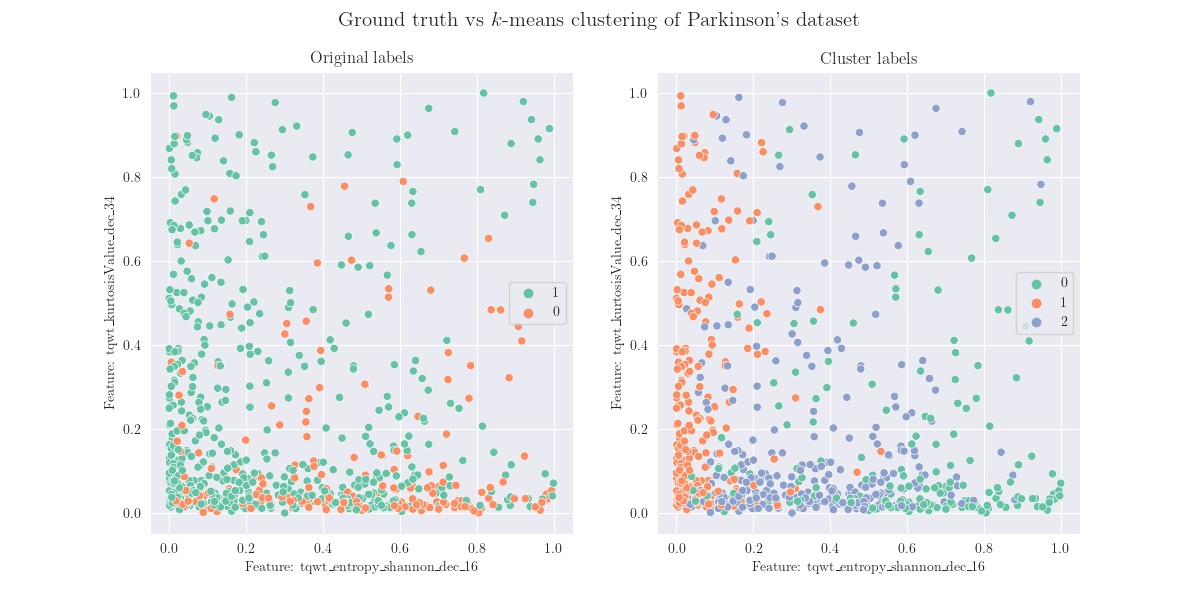
\includegraphics[width=\textwidth]{../assets/parkinsons.png}
  \caption{Ground truth vs $k$-means clustering of Parkinson's dataset}
  \label{fig:diagnoses-plots}
\end{figure}

\end{document}
